% \begin{figure*}[t!]
%     \centering
%     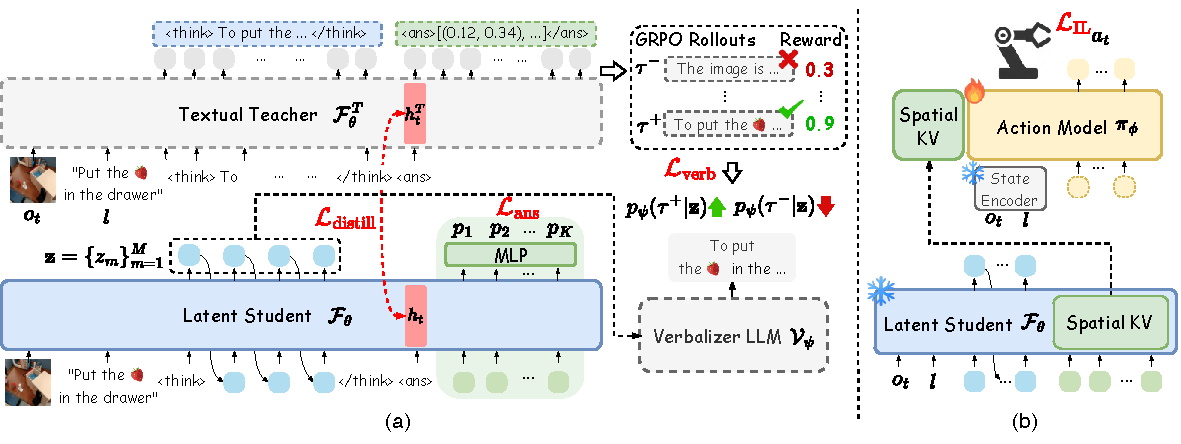
\includegraphics[width=0.95\linewidth]{figures/images/method.pdf}
%     \caption{\textbf{Overview of Fast-ThinkAct.} (a) Given observation $o_t$ and instruction $l$, the Textual Teacher VLM $\mathcal{F}_\theta^T$ generates explicit reasoning chains. The Latent Student VLM $\mathcal{F}_\theta$ distills these into compact latent tokens $\mathbf{z}$ guided by reward preferences. Verbalizer LLM $\mathcal{V}_\psi$ decodes latents to text for preference-based learning via $\mathcal{L}_{\text{verb}}$, while spatial tokens enable parallel visual trajectory prediction via $\mathcal{L}_{\text{ans}}$, ensuring latents are both verbalizable and grounded in visual planning. (b) Reasoning-Enhanced Policy Learning. The trained Latent Student $\mathcal{F}_\theta$ provides reasoning-infused multimodal guidance to the Action Model $\pi_\phi$ for executable action prediction.}
%     \label{fig:method}
%     % \vspace{-2mm}
% \end{figure*}

\begin{figure*}[t!]
    \centering
    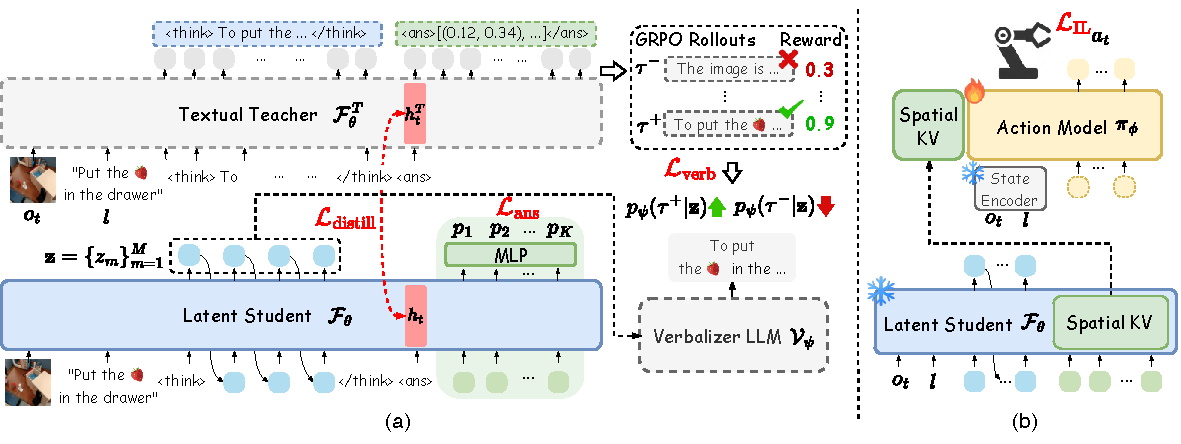
\includegraphics[width=1.0\linewidth]{figures/images/method.pdf}
    \caption{\textbf{Overview of Fast-ThinkAct.} (a) Given observation $o_t$ and instruction $l$, the Textual Teacher VLM $\mathcal{F}_\theta^T$ generates explicit reasoning chains. The Latent Student VLM $\mathcal{F}_\theta$ distills these into compact latent tokens $\mathbf{z}$ guided by reward preferences. Verbalizer LLM $\mathcal{V}_\psi$ decodes latents to text for preference-based learning via $\mathcal{L}_{\text{verb}}$, while $\mathcal{L}_{\text{distill}}$ transfers visual planning capability from teacher, and spatial tokens enable parallel visual trajectory prediction via $\mathcal{L}_{\text{ans}}$, ensuring latents are verbalizable and grounded in visual planning. (b) Reasoning-Enhanced Policy Learning. The Action Model $\pi_\phi$ is trained with $\mathcal{L}_{\text{IL}}$ while freezing the latent student $\mathcal{F}_\theta$ and state encoder.}
    \label{fig:method}
    % \vspace{-2mm}
\end{figure*}
